Before discussing of the improvement of the SFA rate worked out, first we have to formulate what we want to learn from this kind of generalisation. 
In principle we want to investigate how the excited states influence the ionisation process or in general.

We want to investigate what influences the ionization dynamics more, the stark shift or the distortion of the ground state.
This question is being answered here.

However, the much bigger question is that there is quite a big difference between the overall ionization yield from previous simulations within SFA compared with the numerical solution of the TDSE.
An extended version of the SFA model could tell, if the discrepancy is due to the simplification of the dynamics before or after ionization.
% In other words, by including the dynamics before ionization, the remaining difference between the SFA and the TDSE will likely be because of the strong field approximation itself.
% If one would simplify both processes, the only shure information is that both results dont match but one dont know what causes it, the neglection of excited states, SFA itself, or something in between.
Unfortunately, this thesis cannot answer this question to a statisfactory level, but it provides the theoretical framework and formulas needed to achieve this goal in future.





%%%%%%%%%%%%%%%%%%%%%%
\section{Comparison with TDSE using TIPTOE}
First compare the ionization dynamics predicted from the standart SFA approach \cite{Theory_NPS} with the results from tRecX (solving TDSE numerically).
As can be seen in \ref{fig:tiptoe_sfa_comparison}(a), the standart SFA does a good job reconstructing the ionization dynamics, but some parts it does not capture at all\footnote{Note that \eqref{eq:tiptoeprop} is fulfilled and $\delta N(\tau)$ is actually proportional to the signal pulse.}.
Especially in offcycle ionization dyanmics seems to be some kind of phase shift that does not match at all. 

This is the starting point of this thesis since that is what was previously known.
What I implemented is the extended SFA model described in chapter 2 and chapter 4.
As mentioned previously, there are two ways of determining the coefficients, either by solving the TDSE in the subspace of the hilbertspace using the system of ODE`s, or numerically in the full hilbertspace using a numerical solver (here tRecX).
In the plot \ref{fig:tiptoe_sfa_comparison}(b) both the TIPTOE results from the Subspace as well as the Full hilbertspace approach are shown.
Very important is that here, only the first coefficient and first dipole matrix element is used.
In other words, in formula \eqref{eq:sfa_rate_improved} only the first term is used, i.e. $n_1=n_2=1$.
In principle, almost the same formula was already implemented for simulating the standart SFA model, since there is also just the ground state involved.
The only difference is that in the extended SFA model for one state, the coefficient $c_0(t)$ is jused so all the difference between standart SFA and extended SFA in \ref{fig:tiptoe_sfa_comparison}(b) is coming from the coefficients $c_0(t)$.

\medskip
The results show that the extended SFA does indeed show some improvements in reconstructing the offcycle ionization dynamics.
Especially since only the coefficients for the ground state is used, and no excited states are involved, this is a very good result.
Further, as mentioned in more detail in chapter 4, even with the coefficients from the numerical solver, many approximations were made.
Somehow the TIPTOE measurement with coefficients from the subspace do not differ much from the standart SFA model.
\textcolor{red}{why is that the case??}

On the other hand, it seems like there is still some physics missing in the extended SFA model.
Since plot \ref{fig:tiptoe_sfa_comparison}(b) does not include transitions to excited states, this could be a possible reason for the remaining difference.
The other main reason could be that the coulomb potential does indeed play a not negligible role in the ionization process and the small changes in the phase of the ionization yield is coming from that.

\begin{figure}
    \centering
    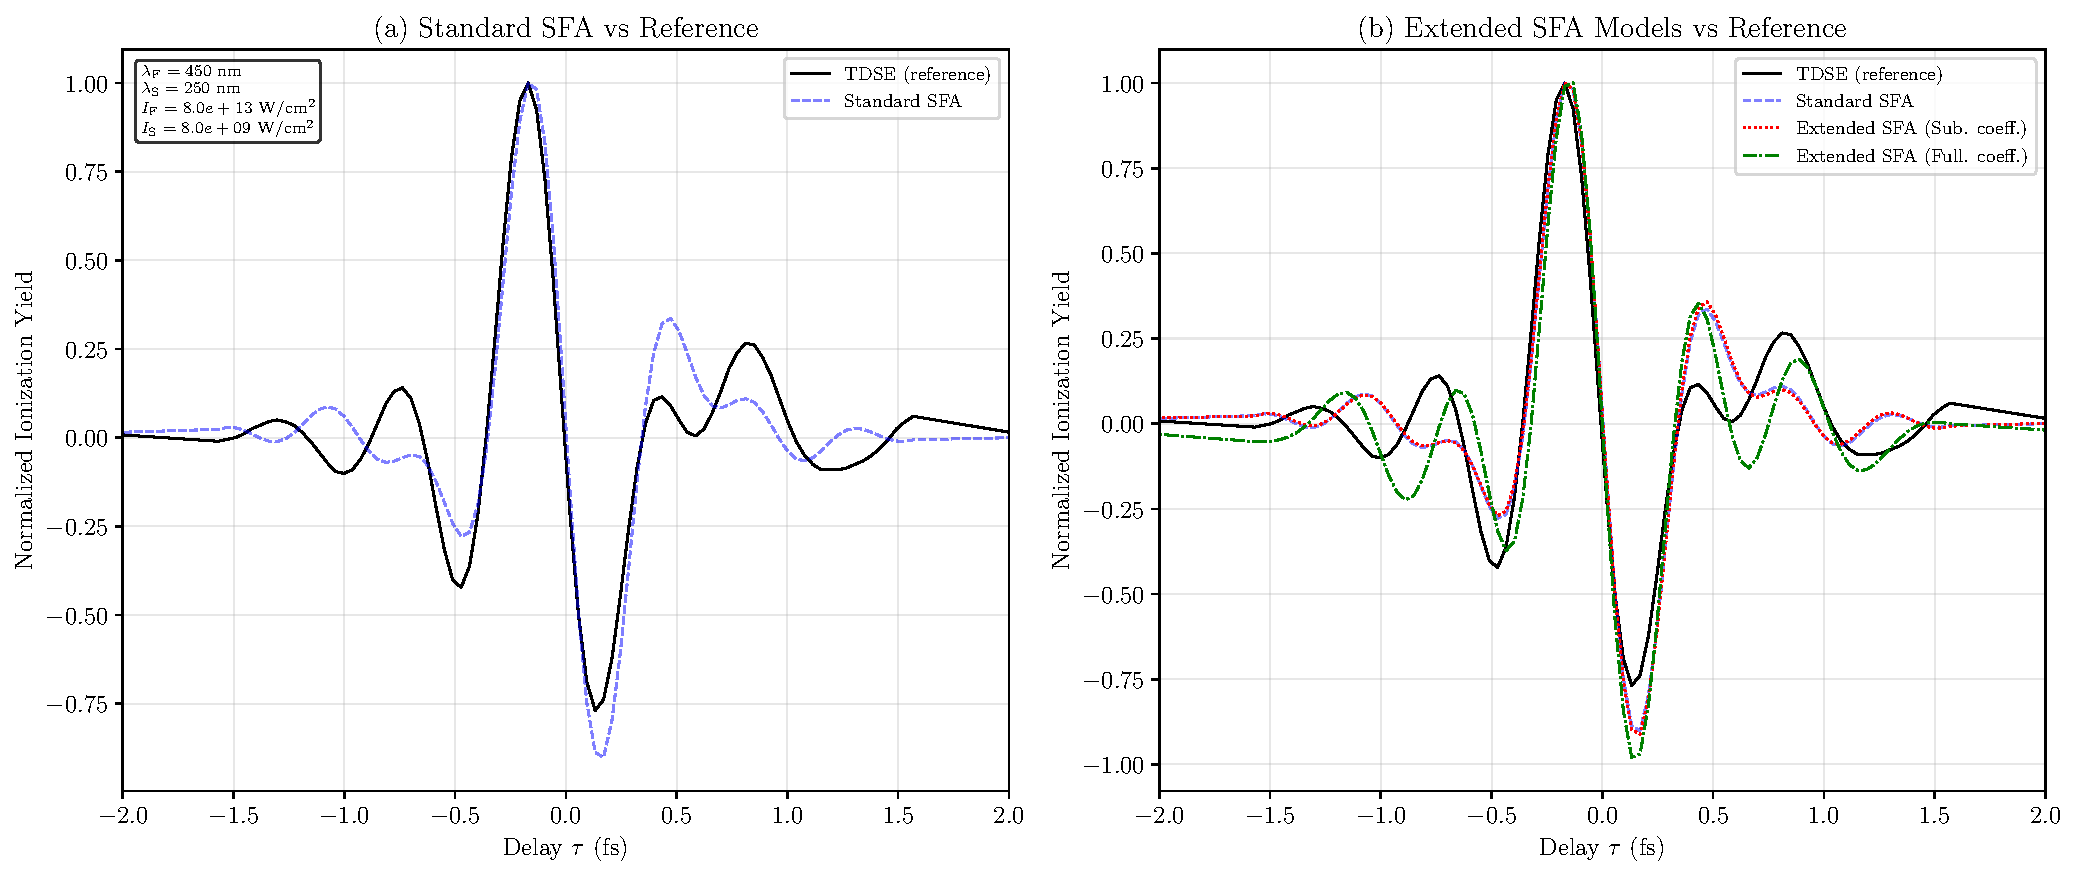
\includegraphics[width=1\textwidth]{../ionModel/python/plotsTIPTOE/2plot_SFA-comparison_1_BA.pdf}
    \caption[Comparison of SFA models and TDSE ionization yields]{Comparison of ionization yields from TIPTOE simulations between different SFA models and reference data from TDSE. 
            (a) Standart SFA overall does a good job reconstructing the ionization dynamics, but some parts it does not capture at all 
            (b) Comparison with extended SFA models with transitions to excited states neglected. }
    \label{fig:tiptoe_sfa_comparison}
\end{figure}


\bigskip
As mentioned in chapter 2, two major physical effects take place that are being carried over by the coefficient $c_0(t)$; the stark shift and the distortion of the ground state. 
By only using the phase of the $c_0(t)$, only the influence of the stark shift is taken into account.
That allows isolating different physical effects and their impact on ionization dynamics.

The figure \ref{fig:tiptoe_rate_stark}(a) shows exactly this approach, a TIPTOE scan but only with the phase of the coefficients:
\begin{equation*}
    c_n(t) = |c_n(t)|e^{i \phi_n(t)} \rightarrow c_n(t) = e^{i \phi_n(t)}
\end{equation*}
The results are obvious.
Almost all the contribution of the imporvement of ionization dynamics within the full hilbertspace coefficients are coming from the change in the energy levels.
This is strong evidence that the stark shift is indeed a very important effect in the ground state ionization dynamics.
The distortion of the ground state does not seem to have much impact.

Figure \ref{fig:tiptoe_rate_stark}(b) shows this in more detail.
In the rates, it is more obvious how much of an contribution the stark shift has in contrast to the distortion of the ground state.





\begin{figure}
    \centering
    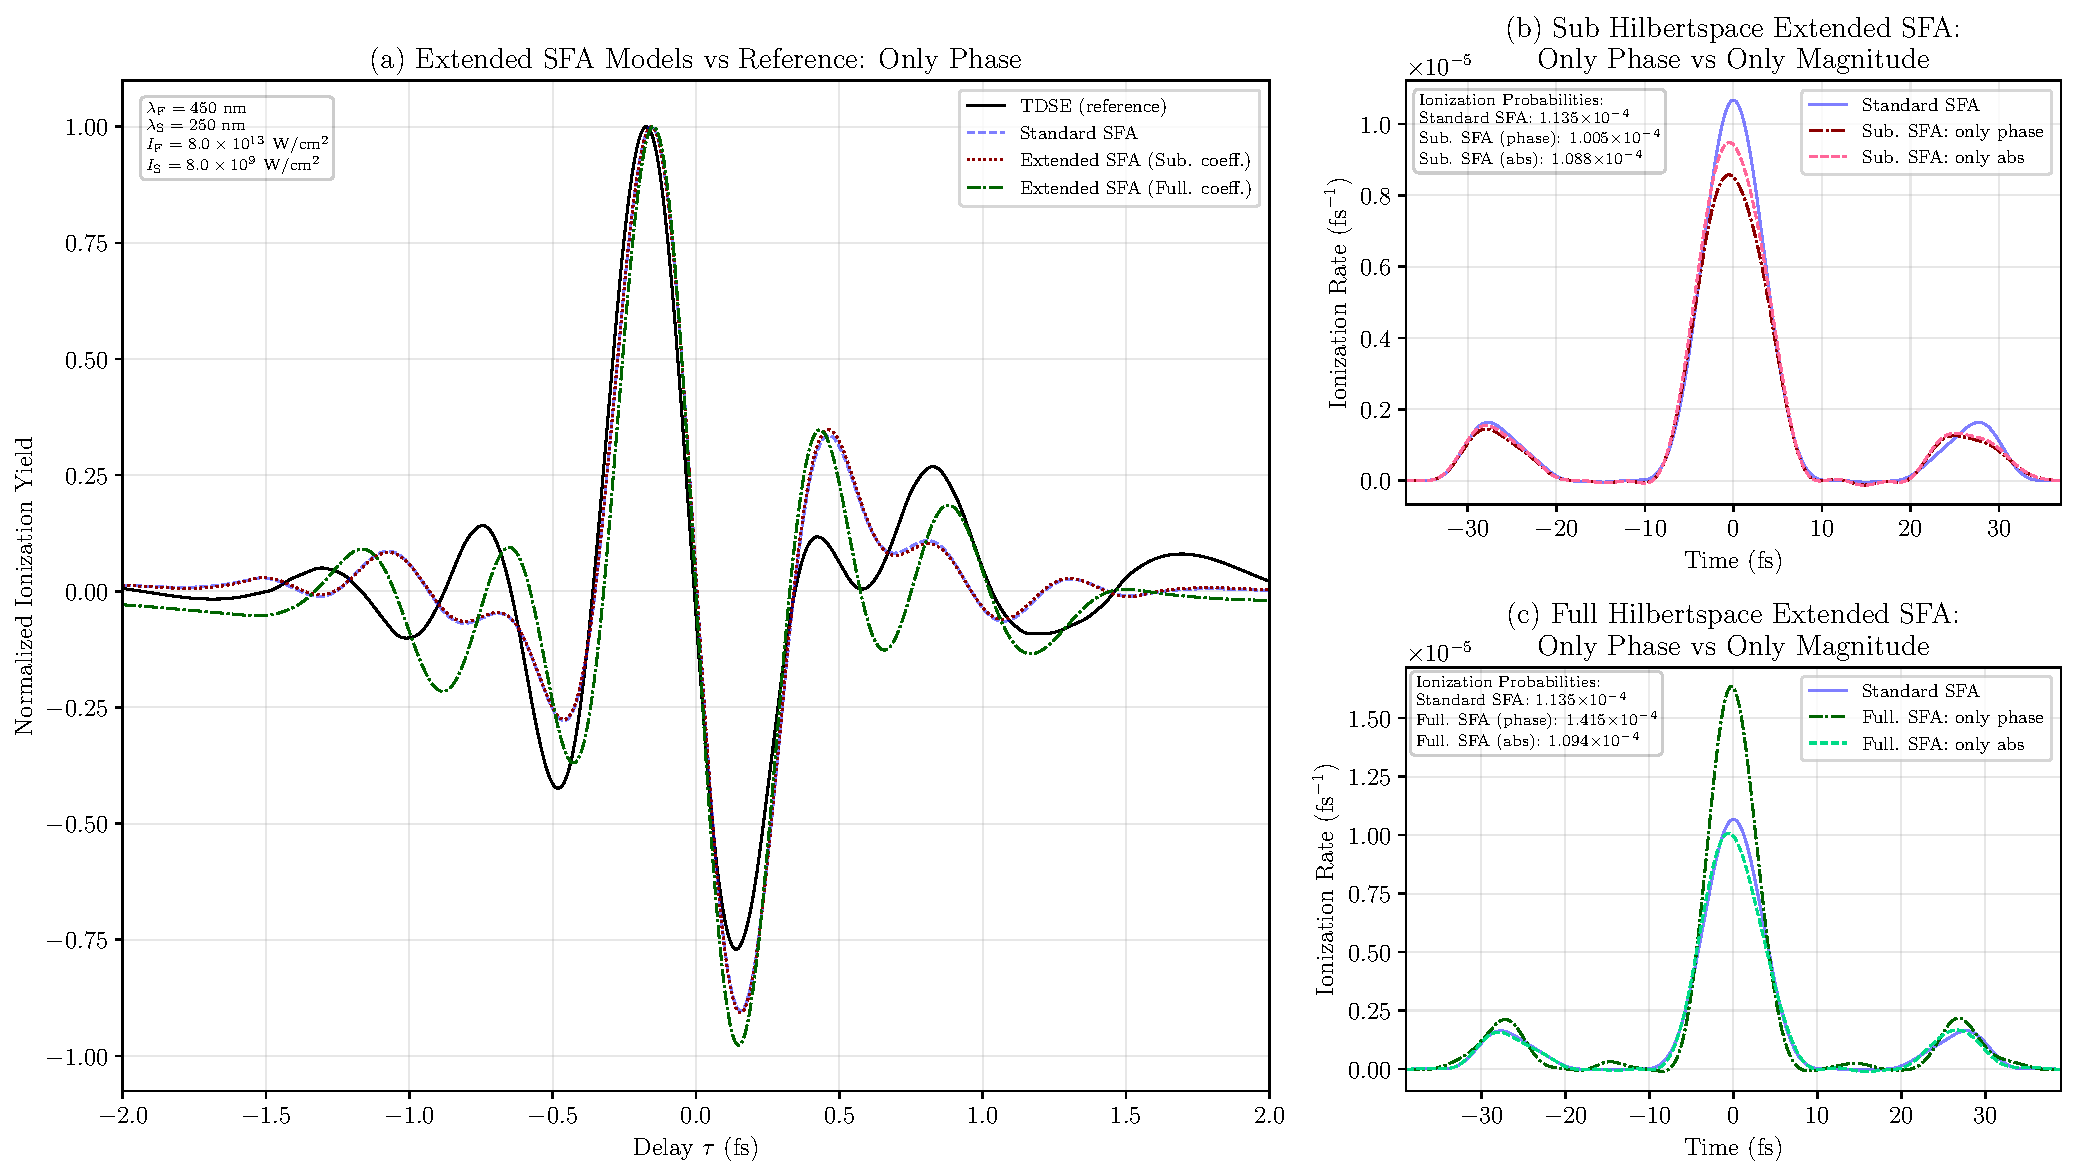
\includegraphics[width=1\textwidth]{../ionModel/python/plotsTIPTOE/3plot_stark-comparison_1_BA.pdf}
    \caption[Impact of stark effect on TIPTOE simulations and ionization rates]{Impact of stark shift on TIPTOE simulations and on ionization rates with transitions to excited states neglected. 
            (a) TIPTOE
            (b) Rate}
    \label{fig:tiptoe_rate_stark}
\end{figure}




\medskip
To make it in one sentence:
Taking only the stark effect of the ground state within the strong field approximation into account while determining the coefficients by solving the TDSE in the full hilbertspace, leads to a better reconstructing of the phase of the ionization dynamics in the offcycle region of the laser pulse than only considering the distortion of the ground state.



\paragraph{Difference in ionization yield between SFA and TDSE}
As mentioned in chapter 3, the Ionization yield in \ref{fig:tiptoe_sfa_comparison} is normalized, to see the actual difference better.
Further, because we are mostly interested in the dynamics and not the plain ionization yield, its normalized according to \eqref{eq:tiptoeprop_normalized}.
However, in the not normalized plot, one could see that the numerical solution of the TDSE is predicting a ionization probability orders of magnitude higher than the SFA model.
In addition to that, small changes in the in the delay of the signal pulse leads to bigger changes in the TDSE results than the SFA results, so the `reference' TIPTOE result is much more sensitive to changes in the laser field.
First observation can be interpreted by the fact that in SFA we are assuming, the electron sits in a continuum state after ionization so the elecotrn does not `feel' the coulomb potential anymore.
This is of course a very strong assumption, any much `harder' to achcieve for the electron. 
Imagine the laser has to really catapult the electron out of the atom to make this assumption approximately valid.
Therefore the overall ionization yield from the SFA model is much lower than the one from the TDSE.
Second, the numerical solution of the TDSE captures much more dynamics and physical effects of the ionization process.
Many different processes can happen during that time, and that could justify why the ionization yield of the TDSE is much more sensitive to changes in the elcetric field.

Both these observations are interesting, but can be expected from how the SFA model is constructed.
To make shure that the differences really do come from the `fundamentals' of the SFA model (i.e. the assumption that the final state is a continuum state), one has to make shure that is the only possible option for the differences.
The extended SFA model described in this thesis may give promising insights into this question.
During the research for this thesis, much work has gotten into the implementation of the extended SFA model, such that it incorparates also excited states .
Unfortunately, due to the limited time frame, I can not present certain results for this question. 
Latest TIPTOE results indicate that including excited states in the SFA rate help to a certain extend the difference in the order of magnitude between SFA and TDSE.
Also the cross-coupling terms in \eqref{eq:sfa_rate_improved} (i.e. $n_1 \neq n_2$) seems to have a significant contribution to the ionizatiion rate.
Furthermore, previous discussed results about the importance of the stark shift applies to excited states as well.
The shift in the energy level of the excited states playes a more significant role for the ionization rate than changes in the probability ampltidue of the coefficients.
The indicated changes in the order of magnitude of the ionization yield that could come from including excited states in the extended SFA model is could primarily coming from the dipole transition matrix elements.
For example this could be explained by the lase rpulse exciting the elctron to for isnatnce the 3p state and later ionizing it.
This will result in a much hgiher ionization probability overoll since more is possible.
However, this could not be shown here.
But these are not really results, only some hints.

















% On the left plot we see that tRecX is still orders of magnitude larger than the SFA results. 
% However, with excited states it goes in the right direction as can be seen on the right plot. 
% For three excited sates there is not much imporvement visible.
% Unfortunately, the results are no where close to the tRecX measurements. That indicates that there is some physics missing in the SFA model.
% If its not the excited states, the it must be something else.
% And because the change is so big it has to be something more fundamental.
% The first idea is that the interaction with the coulomb potential after ionization cannot be completely neglected, as it is done in the SFA model.
% Even though it is counterintuitive, becasue if the coulomb potential is still noticable for the electron after ionization, why would it increase the results we are seeing??????
% But this is in principle what our simulations are telling us. We can argue that we have two different ways of calculating the coefficients (ODE and tRecX) and the reproduce the same result.

% However it indicates that real ionization propabilities do have some characterisitcs that the improved SFA model does not capture.

% One also should make clear what the ODE coefficients do not capture. First, I implemented the code such that it ignores transitions not allowed by the dipole selection rules.

% So in principle, assuming my SFA modification was correct the TIPTOE results tell us that the coulomb potential is not negligible after all. 
% Maybe because the laser is not that intense (multiphoton ionization).
% But its difficult to test that because if I increase the laser intensity, the approximations I made with the coefficients is not valid anymore.

% Looking at not normalized results, tRecX is much more sensitive to the shift of probe and pump pulse, while excited SFA coefficients are not
% Maybe because tRecX takes into account all the dynamics and effects inside an atom, while excited SFA coefficients does not care that much.
% I would expect with tRecX coefficients more sensitive than with ODE coefficients???

% \section{Influence of Stark Shift and Polarisation}
% The Stark effect is the shift of the energy levels of an atom or molecule due to the presence of an external electric field.

% \begin{figure}[H]
%     \centering
%     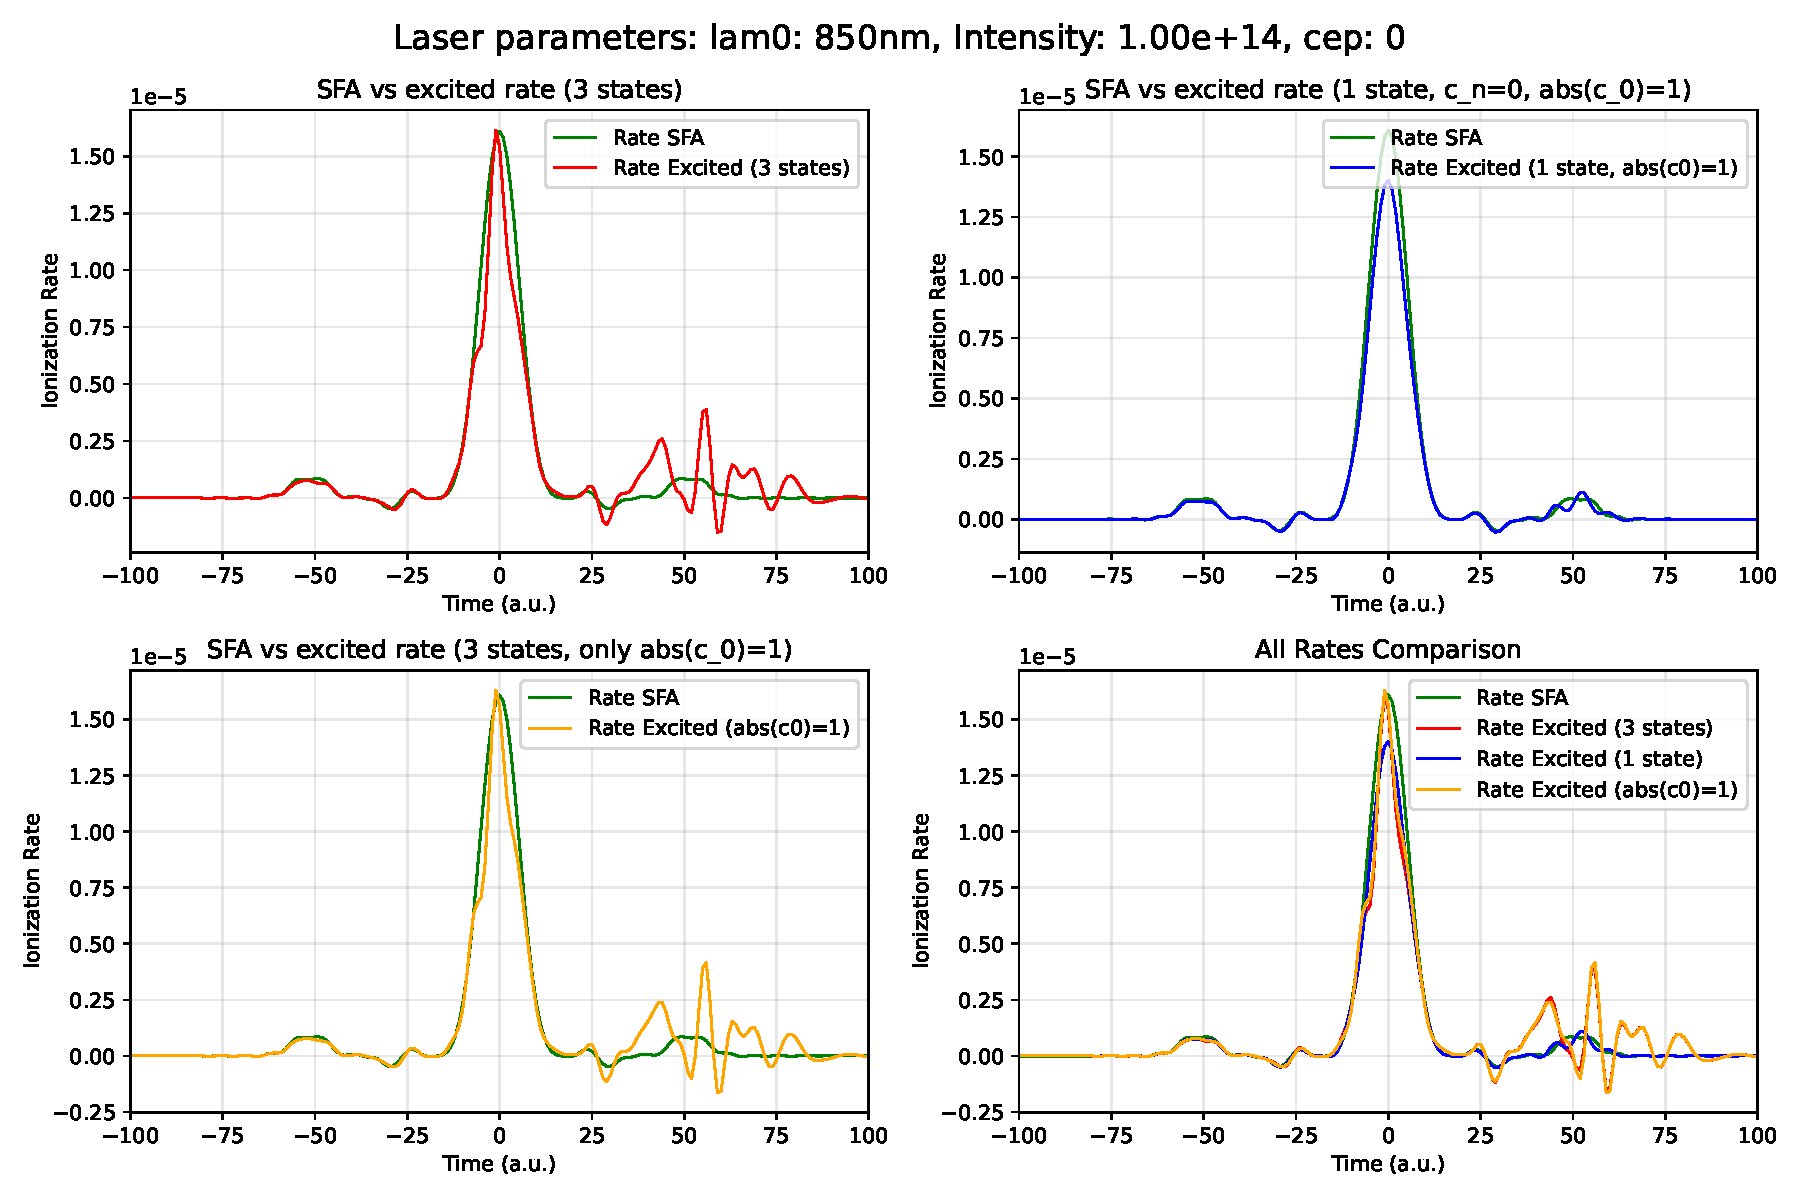
\includegraphics[width=0.9\textwidth]{figures/rate4_850_1.00e+14_onlystark.pdf}
%     \caption{stark effect}
%     \label{fig:starkeffect}
% \end{figure}

% Naiv: Stark effect changes energy in electron so its "harder" to ionise, thats why blue curve goes down (when excitedStates=1). 
% But thats not certainly the case because of stark effect, thats why only set absc0 to 1 and phase remains. 
% Example with oszillations with time dependent resonance frequency, and external force not at resonance but coincidence with oszillator resonance frequency so this may cause it.

% \bigskip
% Stark shift doesnt seem to have much contribution (sadly) but at least more than the polarisation of the ground state.

% Lets investigate the influence of first coefficient, nothing more. Only the phase has a contribution, the amplitude is not important.
% Thats because the amplitude determines something occupation propabilitiy, but the phase is $e^{-iEt}$ and if $E$ is shifted by a bit you can isolate it by just using purely the phase.\\
% Top right is the isolated stark effect








% \section{Laser Fields}
% Lorem ipsum dolor sit amet, consetetur sadipscing elitr, sed diam nonumy eirmod tempor invidunt ut labore et dolore magna aliquyam erat, sed diam voluptua. At vero eos et accusam et justo duo dolores et ea rebum. Stet clita kasd gubergren, no sea takimata sanctus est Lorem ipsum dolor sit amet. Lorem ipsum dolor sit amet, consetetur sadipscing elitr, sed diam nonumy eirmod tempor invidunt ut labore et dolore magna aliquyam erat, sed diam voluptua. At vero eos et accusam et justo duo dolores et ea rebum. Stet clita kasd gubergren, no sea takimata sanctus est Lorem ipsum dolor sit amet.


% \begin{equation}
%     \partial_t u = \mathcal{H}(t)  \lambda 
% \end{equation}

% \begin{figure}[H]
%     \centering
%     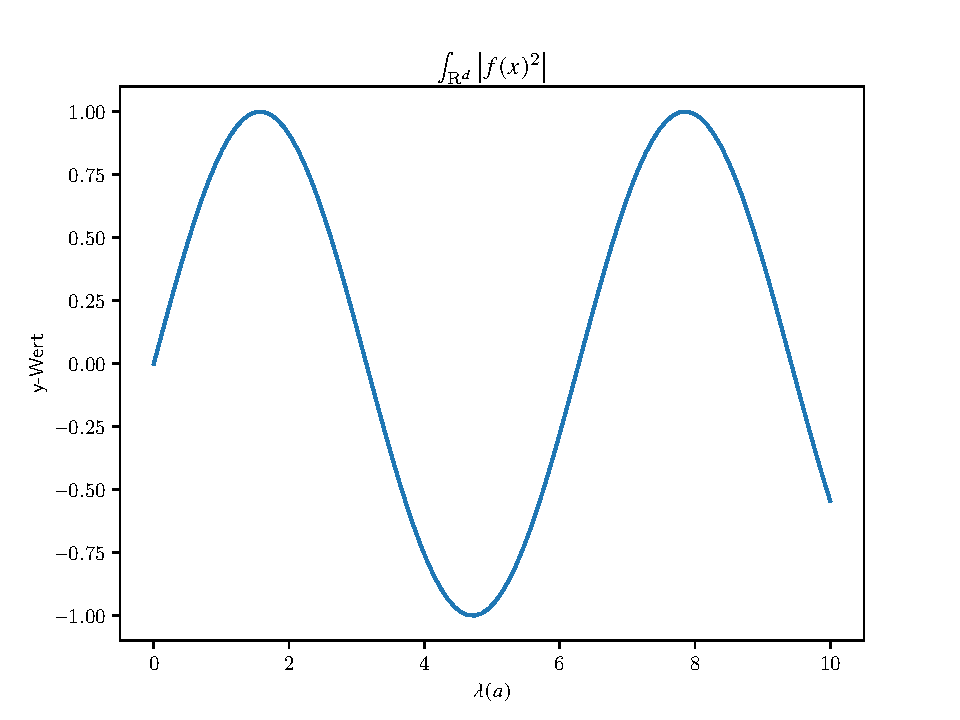
\includegraphics[width=0.5\textwidth]{figures/plot.pdf}
%     \caption{Sine function}
%     \label{fig:sinus}
% \end{figure}



% \begin{equation*}
%     \partial \A = \B
% \end{equation*}

% \medskip

% \begin{equation}
%     \int_{\R^d} \abs{f(x)}^2 \dd x = \int_{\R^d} \abs{\F f(\xi)}^2 \dd \xi
% \end{equation}

% \medskip

% \begin{equation}
%     %schrödinger equation
%     \ii \partial_t u = \mathcal{H}(t) \Ket{a} \lambda 
% \end{equation}

% \begin{equation}
%     \gimel \overrightarrow{a} \cos \mathrm{cos} \Rightarrow \Longrightarrow \nearrow 
% \end{equation}
